\documentclass[a4paper,11pt]{article}

\usepackage[utf8]{inputenc} \usepackage[T1]{fontenc}
\usepackage{fancyhdr} \usepackage{graphicx,subfig} \usepackage{lastpage}
\usepackage{amssymb,amsmath} \usepackage{siunitx} \usepackage[nodayofweek]{datetime}
\usepackage[top=3.5cm,bottom=2.5cm,left=3cm,right=3cm,headheight=40pt]{geometry}
\usepackage{parskip} \usepackage{float} \usepackage{enumitem} \pagestyle{fancy}
\usepackage[colorlinks=true,allcolors=blue]{hyperref} \hypersetup{
	pdfauthor={Michaël Defferrard},
	pdftitle={Project stage 1: Terrain generation},
	pdfsubject={Introduction to Computer Graphics}
}

\lhead{Introduction to Computer Graphics\\Project stage 1: Terrain generation\\Group 19}
\chead{\hspace{2.5cm}EPFL\\\hspace{2.5cm}\shortdate\today\\\hspace{2.5cm}\thepage/\pageref{LastPage}}
\rhead{Michaël \textsc{Defferrard}\\Pierre \textsc{Fechting}\\Vu Hiep \textsc{Doan}}
\cfoot{}

\begin{document}


\section{Overview}


\begin{figure}[ht]
	\centering
	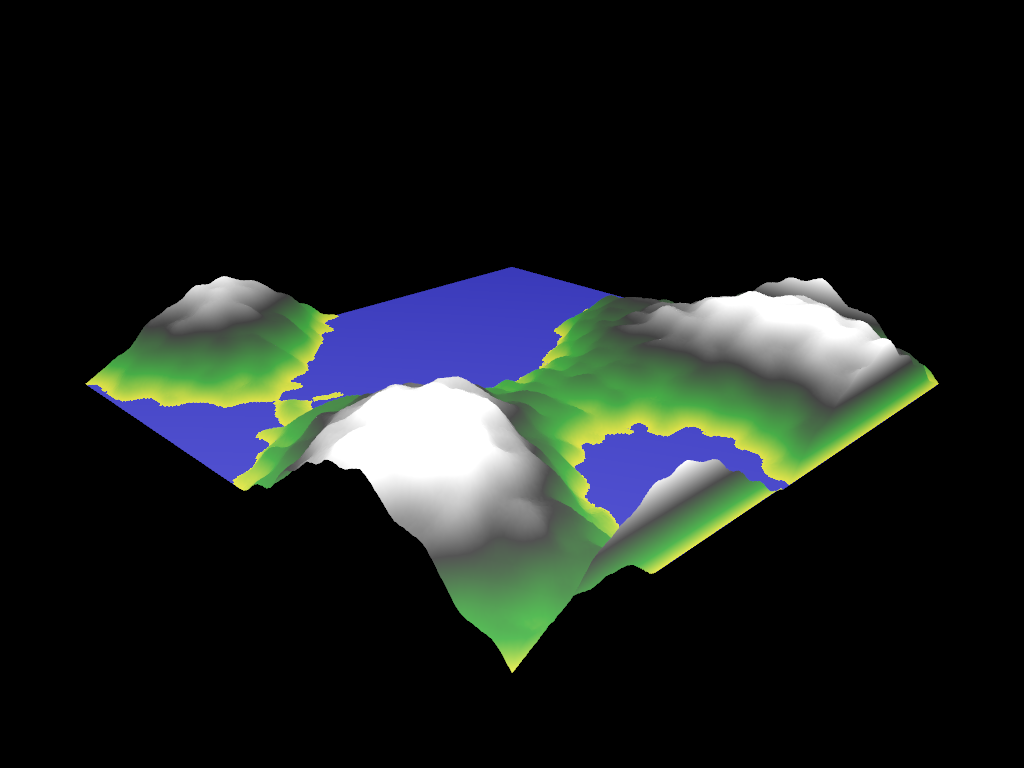
\includegraphics[height=7cm]{{{img_stage1/fBm_1.1_10.0_10_2.0_withZeroGrad}}}
	\caption{Example terrain generated by fractal Brownian motion with $H=1.1$, $l=10$ and 10 octaves.}
	\label{fBm}
\end{figure}



\section{Implementation}

\subsection{Triangle grid}

We first generate the flat triangle mesh as a base for our terrain. The implementation is quite straightforward for a grid of size $N \times N$ as first, two VBOs storing the positions of each vertex and the corresponding faces' indices also are calculated.

We then render it as a triangle mesh by function \texttt{glDrawElements} to get a smooth triangle mesh (see 		~\ref{triangle_grid_full}). It is also worth noticing the use of \texttt{glPolygonMode}, which allows us to render only the triangles' boundaries as shown in figures~\ref{triangle_grid_8}, \ref{triangle_grid_16} and~\ref{triangle_grid_64} for $N=8$, $N=16$ and $N=64$, respectively.

\begin{figure}[ht]
	\centering
	\subfloat[Lines with $N=8$]{
		\label{triangle_grid_8}
		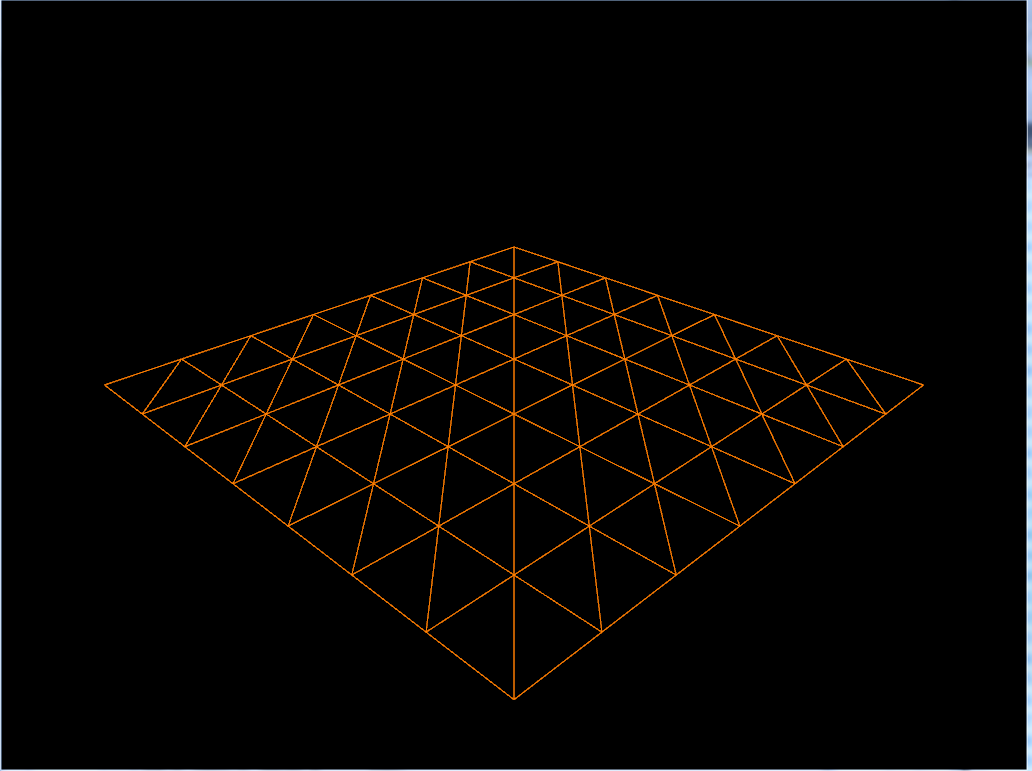
\includegraphics[height=4cm]{{{img_stage1/triangle_grid_8}}}
	} \quad
	\subfloat[Lines with $N=16$]{
		\label{triangle_grid_16}
		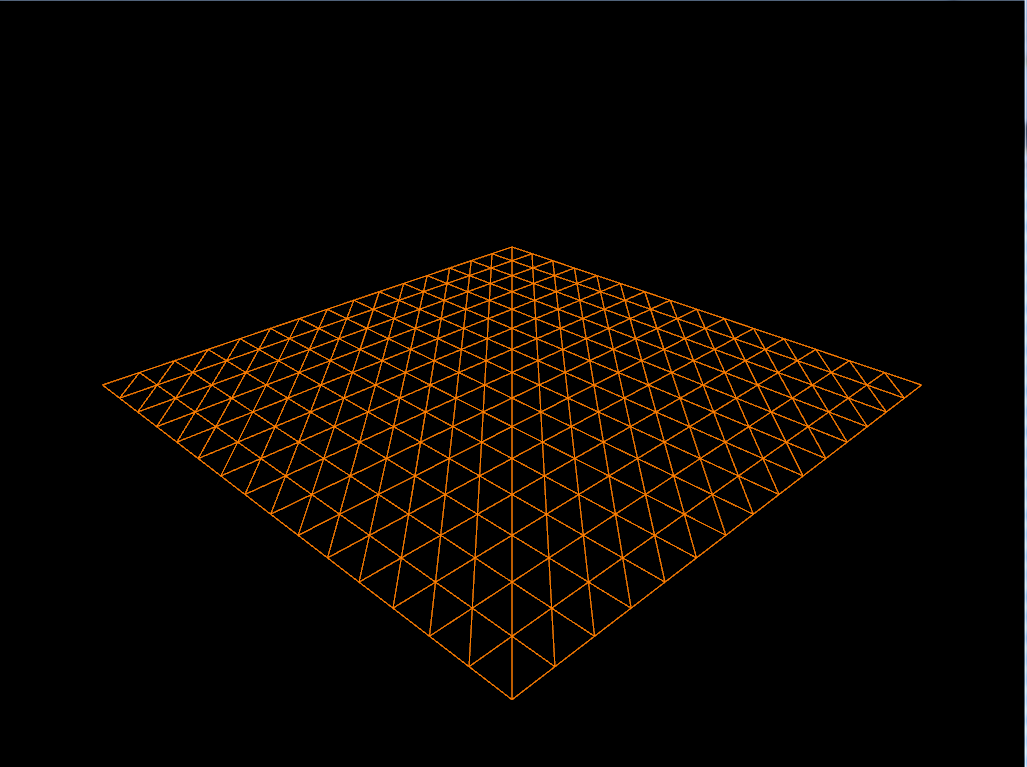
\includegraphics[height=4cm]{{{img_stage1/triangle_grid_16}}}
	} \quad
	\subfloat[Lines with $N=64$]{
		\label{triangle_grid_64}
		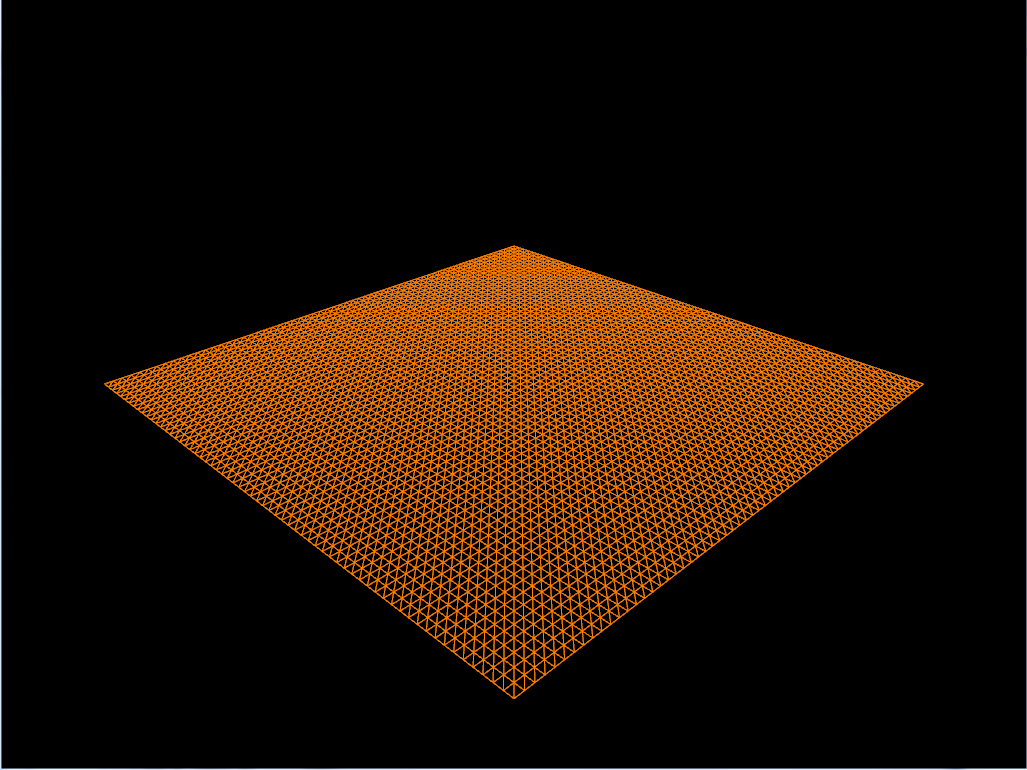
\includegraphics[height=4cm]{{{img_stage1/triangle_grid_64}}}
	} \quad
	\subfloat[Triangles]{
		\label{triangle_grid_full}
		
\includegraphics[height=4cm]{{{img_stage1/triangle_grid_full}}}
	}
	\caption{Triangle grid}
	\label{triangle_grid}
\end{figure}

\subsection{Diffuse shading}
The terrain generated from displacing each vertex in base triangle grid according to height map will be applied the diffuse shading for better visualization. In short, each vertex will be colored by the result value of following equation: $I_dk_d(N\cdot L)$ where $I_d$ and $k_d$ is the diffuse color of the light source and material, respectively. $N$ is the normal vector at that vertex and $L$ is the normalized light direction vector.

We define te diffuse color of light source and material as well as the light position so except $N$, other values are very easy to compute. For calculating normal vector $N$, we use finite difference to approximate a gradient vectors $\nabla x$ and $\nabla y$ along \textit{x} and \textit{y} directions. Note that to compute theses gradients, we need the elevation at four neighboring vertices as well, which can be done again by looking up on the height map that we generated.

Then, the normal vector will be cross product of $\nabla x$ and $\nabla y$. 

\subsection{Height map}

We did first construct an heightmap by hand (\texttt{gen\_test\_height\_map}) with a 3x3 pixels texture to test the displacement procedure of the rendering vertex shader and the height sensible coloring of the rendering fragment shader (fig.~\ref{test_heightmap}). We then implemented the texture rendering (\texttt{gen\_height\_map}). To test the framework, we rendered a simple texture of 1024x1024 pixels which all have the value of 0.5 (fig.~\ref{test_heightmap_gen}).

\begin{figure}[ht]
	\centering
	\subfloat[Heightmap constructed by hand]{
		\label{test_heightmap}
		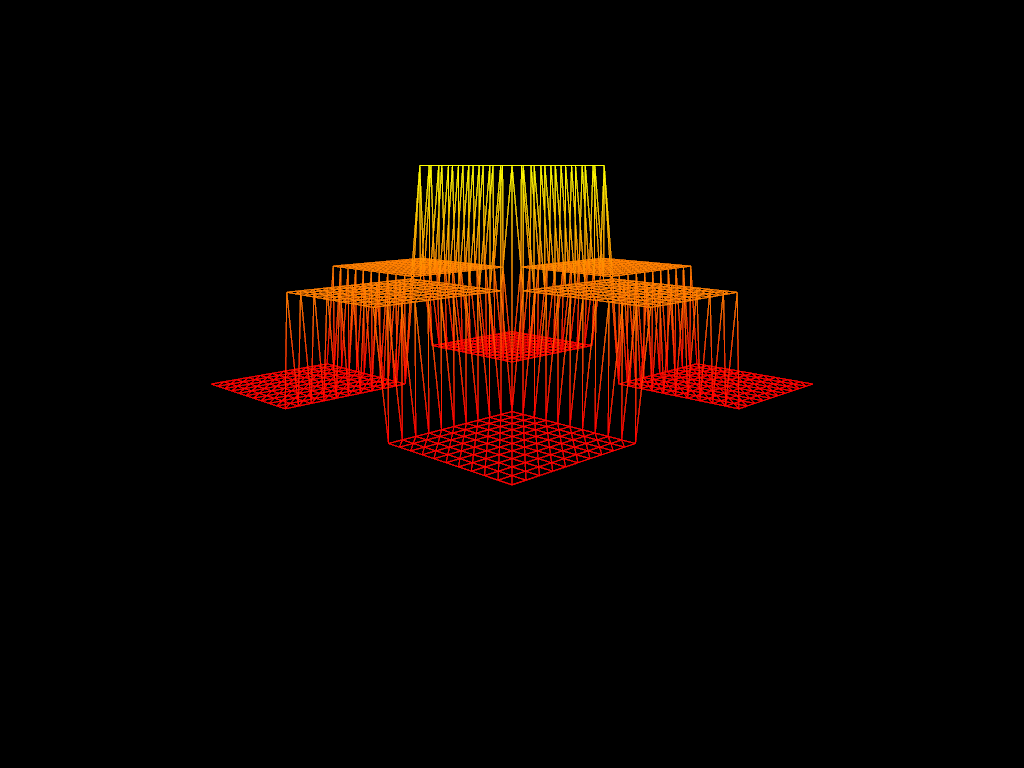
\includegraphics[height=4cm]{{{img_stage1/test_heightmap}}}
	} \quad
	\subfloat[Simple generated heightmap]{
		\label{test_heightmap_gen}
		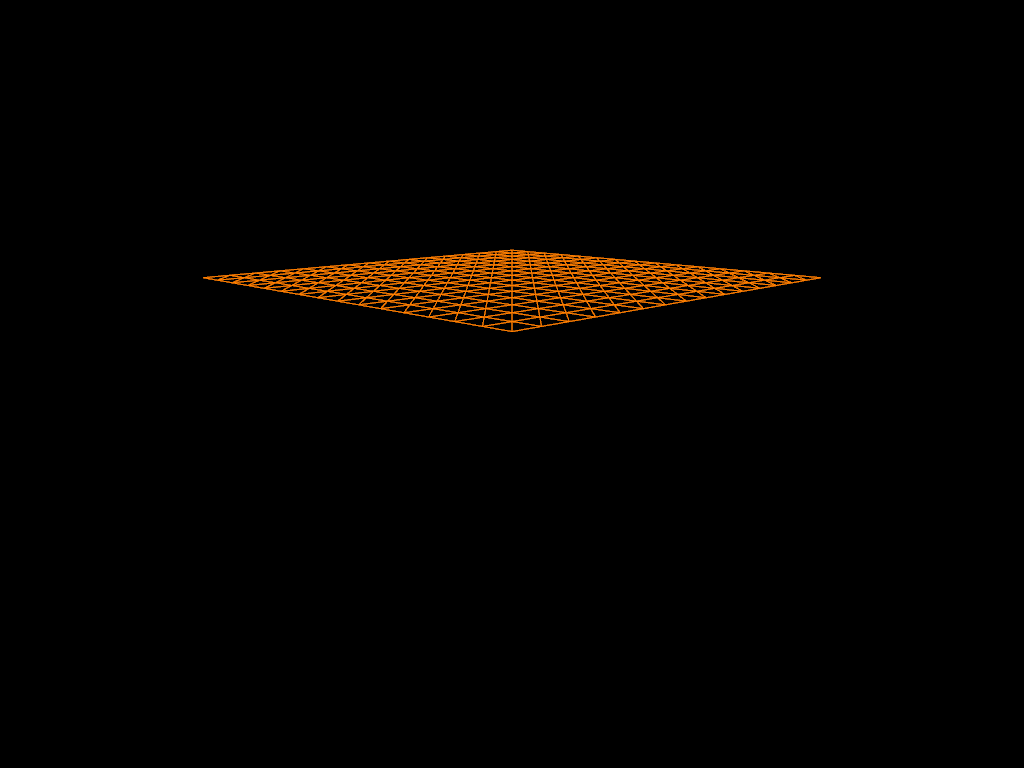
\includegraphics[height=4cm]{{{img_stage1/test_heightmap_gen}}}
	}
	\caption{Heightmaps}
\end{figure}

\subsection{Perlin noise}

We then implemented the Perlin noise in the heightmap fragment shader. As suggested by the tutorial linked in the hand-out, we used a permutation table to generate a pseudo-random number per square.

indexed texture access instead of interpolation in normalize coordinates

Show some screenshots with different frequencies and amplitudes of the noise function.

With / without zeros in gradients.

\section{Results}



\end{document}
